\documentclass[../deliverable-two.tex]{subfiles}

\begin{document}
\label{architecture}

Przedstawiony system składa się z następujących modułów:
\begin{itemize}
	\item nadzorcy,
	\item serwer wirtualizacji,
	\item brokera wiadomości,
	\item aplikacji klienckiej,
	\item panelu administratora,
	\item systemu katalogowego,
	\item dysku współdzielonego.
\end{itemize}
Schematyczny obraz systemu przedstawia poniższy rysunek.

\begin{figure}[!h]
	
	\centering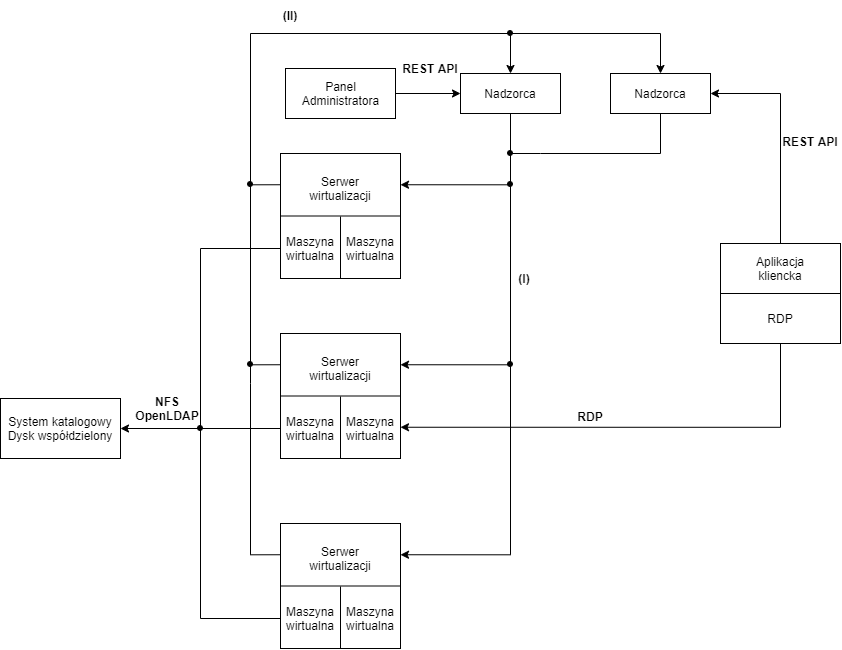
\includegraphics[width=\screenswidth]{architecture.png}
	
	\vskip-1.5ex
	
	\caption{Schematyczna architektura systemu}
	\label{obrazek}
\end{figure}

Z założenia system powinien móc skalować się w dwóch wymiarach, to znaczy:
\begin{enumerate}
	\item Zwiększanie liczby serwerów wirtualnych - zwiększenie liczby sesji dla użytkowników.
	\item Zwiększenie liczby nadzorców - zwiększenie liczby obsługiwanych klientów jednocześnie.
\end{enumerate}

Szczegółowe opisy poszczególnych modułów będą omówione w następnych rozdziałach: \nameref{modules} oraz \nameref{external-modules}.

\end{document}